\documentclass[twoside]{article}
\usepackage[a4paper]{geometry}
\geometry{verbose,tmargin=2.5cm,bmargin=2cm,lmargin=2cm,rmargin=2cm}
\usepackage{fancyhdr}
\pagestyle{fancy}

% nastavení pisma a~češtiny
\usepackage{lmodern}
\usepackage[T1]{fontenc}
\usepackage[utf8]{inputenc}
\usepackage[czech]{babel}

% odkazy
\usepackage{url}

\usepackage{float}
% vícesloupcové tabulky
\usepackage{multirow}
\usepackage{listings}
\usepackage{xcolor}
\usepackage{amssymb}
\usepackage{gensymb}
\usepackage{bbold}
\usepackage{amsmath}
\usepackage{siunitx}
\usepackage{mathtools}
\usepackage{commath}

% vnořené popisky obrázků
\usepackage{subcaption}

% automatická konverze EPS 
\usepackage{graphicx} 
\usepackage{epstopdf}
\epstopdfsetup{update}

\graphicspath{{./images}}

% odkazy a~záložky
\usepackage[unicode=true, bookmarks=true,bookmarksnumbered=true,
bookmarksopen=false, breaklinks=false,pdfborder={0 0 0},
pdfpagemode=UseNone,backref=false,colorlinks=true] {hyperref}


% Poznámky při překladu
\usepackage{xkeyval}	% Inline todonotes
\usepackage[textsize = footnotesize]{todonotes}
\presetkeys{todonotes}{inline}{}

%https://tex.stackexchange.com/questions/2783/bold-calligraphic-typeface
\DeclareMathAlphabet\mathbfcal{OMS}{cmsy}{b}{n}

% enumerate zacina s pismenem
\renewcommand{\theenumi}{\alph{enumi}}

% smaz aktualni page layout
\fancyhf{}
% zahlavi
\usepackage{titling}
\fancyhf[HC]{\thetitle}
\fancyhf[HLE,HRO]{\theauthor}
\fancyhf[HRE,HLO]{\today}
 %zapati
\fancyhf[FLE,FRO]{\thepage}

% údaje o autorovi
\title{OTE Domácí úkol 4b - Vzorkovací zesilovač}
\author{Vojtěch Michal}
\date{\today}

%customize code listing
\definecolor{codegreen}{rgb}{0,0.6,0}
\definecolor{codegray}{rgb}{0.5,0.5,0.5}
\definecolor{codepurple}{rgb}{0.58,0,0.82}
\definecolor{backcolour}{rgb}{0.95,0.95,0.92}

\lstdefinestyle{mystyle}{
    backgroundcolor=\color{backcolour},   
    commentstyle=\color{codegreen},
    keywordstyle=\color{magenta},
    numberstyle=\tiny\color{codegray},
    stringstyle=\color{codepurple},
    basicstyle=\ttfamily\footnotesize,
    breakatwhitespace=false,         
    breaklines=true,                 
    captionpos=b,                    
    keepspaces=true,                 
    numbers=left,                    
    numbersep=5pt,                  
    showspaces=false,                
    showstringspaces=false,
    showtabs=false,                  
    tabsize=2
}

\lstset{style=mystyle}

\begin{document}

\maketitle

V simulacích pro tuto úlohu bylo použito nastavení parametrů operačních zesilovačů a spínače uvedené v tabulce \ref{tab:oz_param}.
Symbolem $u_2$ označuji napětí na výstupu vzorkovacího zesilovače proti zemi,
napětí $u_1$ je napětí na vstupu vzorkovacího zesilovače proti zemi
(konvence použitá v zadání).

\begin{table}[h!]
    \centering
    \begin{tabular}{c|c|c|c|c}
        parametr & symbol & hodnota & jednotka & poznámka\\
        \hline
        Vstupní napěťový offset & $U_0$ & 1 & \si{\milli\volt} & \\
        Vstupní klidový proud & $I_\text{B}$ & 50 & \si{\nano\ampere} & $(I_\text{BP} + I_\text{BN})/2$ \\
        Vstupní zbytkový proud & $I_0$ & 20 & \si{\nano\ampere} & $I_\text{BP} - I_\text{BN}$ \\
        Zesílení v otevřené smyčce & $A_\text{D}$ & 200 & \si{\kilo\volt\per\volt} & \\
        Tranzitní kmitočet& $f_T$ & 1 & \si{\mega\hertz} & \\
        odpor S1 v sepnutém stavu & $R_\text{on}$ & 10 & \si{\milli\ohm} & \\
        odpor S1 v rozpenutém stavu & $R_\text{off}$ & 1 & \si{\giga\ohm} & \\
    \end{tabular}
    \caption{Parametry obvodu použité pro simulaci}
    \label{tab:oz_param}
\end{table}

\section{Převodní charakteristika}

Pro měření bylo použito zapojení na obrázku \ref{fig:prevodni_char_schema},
na kterém je i vidět změřené výstupní klidové napětí $U_{20} = 200 \si{\micro\volt}$.
Převodní charakteristika v režimu sledování je vykreslena na obrázku \ref{fig:prevodni_char},
zesílení obvodu je na celém rozsahu vstupů jedničkové.


\begin{figure}[h!]
    \centering
    \includegraphics[width=0.65\linewidth]{zbytkove_vystup.png}
    \caption{Schéma pro měření převodní charakteristiky}
    \label{fig:prevodni_char_schema}
\end{figure}

\begin{figure}[h!]
    \centering
    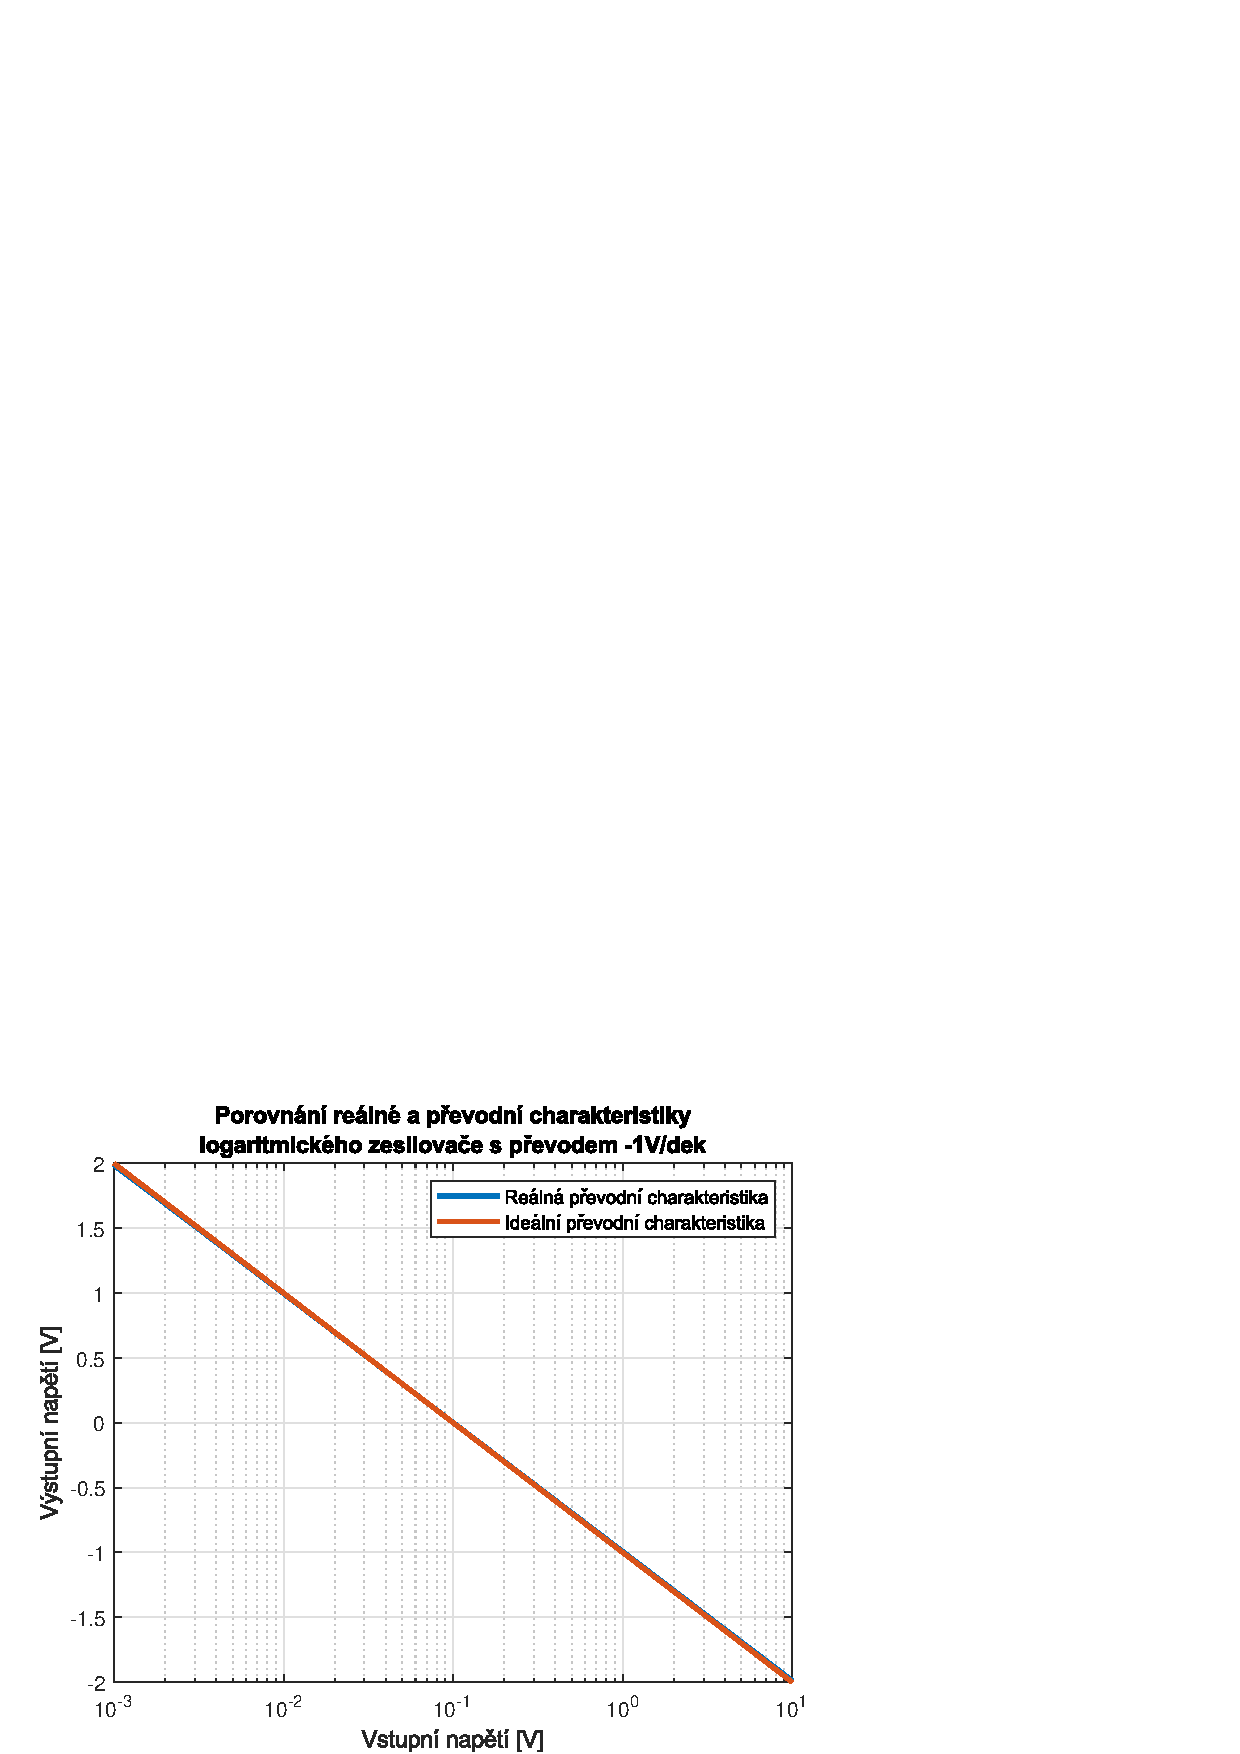
\includegraphics[width=0.4\linewidth]{prevod_char.pdf}
    \caption{Převodní charakteristika vzorkovacího zesilovače v režimu sledování}
    \label{fig:prevodni_char}
\end{figure}

Díky jedničkovému zesílení je i vstupní klidové napětí rovno $U_{10} = 200 \si{\micro\volt}$.
Toto je ověřeno pomocí zpětnovazebního zapojení na obrázku \ref{fig:vstupni_zbytkove}.

\begin{figure}[h!]
    \centering
    \includegraphics[width=0.55\linewidth]{zbytkove_u.png}
    \caption{Zapojení pro měření vstupního zbytkového napětí}
    \label{fig:vstupni_zbytkove}
\end{figure}

\newpage
\section{Frekvenční charakteristika v režimu pamatování}


\begin{figure}[h!]
    \centering
    \includegraphics[width=0.55\linewidth]{bode_schema.png}
    \caption{Zapojení pro získání frekvenční charakteristiky vzorkovacího zesilovače}
    \label{fig:schema_bode}
\end{figure}

S pomocí zapojení na schématu \ref{fig:schema_bode} a funkce \textit{AC sweep} byly
získány frekvenční charakteristiky pro $C_H \in \left\{10, 1000\right\} \si{\nano\farad}$,
které jsou vykresleny na obrázkách \ref{fig:bode_10} a \ref{fig:bode_1000}.
Na grafech jsou kurzory vyznačené vždy dva průběhy -- červenou barvou je vyvedeno
napětí na uzlu 1 (výstup vzorkovacího zesilovače), zatímco zelenou je napětí na uzlu 6
(paměťový kondenzátor). Průběh na výstupu odpovídá standardnímu zesilovači s jedničkovým
zesílením. Charakteristika je plochá na úrovni 0 dB až do mezního kmitočtu použitých OZ.

Naopak průběh na paměťovém kondenzátoru se zalomí dříve, neboť jeho mezní frekvence
je obecně $f_m = (2\pi R_2 C_H)^{-1}$, což dává $f_m = 53 \si{\kilo\hertz}$ pro $C_H = 10 \si{\nano\farad}$
a $f_m = 530 \si{\hertz}$ pro $C_H = 1 \si{\micro\farad}$. Tomuto výpočtu odpovídají
i mezní frekvence odečtené pomocí kurzorů.
Pro reálné použití tohoto vzrokovacího zesilovače je potřeba sledovat zejména zelenou křivku,
protože ona udává, jak se bude výstup chovat, začneme-li periodicky rozepínat spínač S1
a tedy odpojovat tvrdý zdroj vstupního napětí v podobě výstupu Z1.


\newpage
\begin{figure}[h!]
    \centering
    \includegraphics[width=0.92\linewidth]{bode_10.pdf}
    \caption{Frekvenční charakteristika pro $C_1 = 10 \si{\nano\farad}$}
    \label{fig:bode_10}
\end{figure}

\begin{figure}[h!]
    \centering
    \includegraphics[width=0.92\linewidth]{bode_1000.pdf}
    \caption{Frekvenční charakteristika pro $C_1 = 1000 \si{\nano\farad}$}
    \label{fig:bode_1000}
\end{figure}

\newpage
\section{Doba náběhu a ustálení}
\label{sec:rise}
\begin{figure}[h!]
    \centering
    \includegraphics[width=0.7\linewidth]{rise_time_schema.png}
    \caption{Zapojení pro měření doby náběhu a ustálení}
    \label{fig:rise_schema}
\end{figure}

S pomocí generátoru obdélníkového signálu a osciloskopu zapojeného dle schématu \ref{fig:rise_schema}
byly zachyceny časové průběhy vykreslené na obrázkách \ref{fig:doby} pro $C_1 = 1 \si{\micro\farad}$.

Doba náběhu $T_n = 495 \si{\nano\second}$ je delší než teoreticky vypočtená $T_n \approx 0,35/f_m \approx 350 \si{\nano\second}$,
což lze vysvětlit konečnou rychlostí přeběhu OZ. Ustálení na 5 \% nastává po čase $T_s = 650 \si{\nano\second}$.
Tyto hodnoty \underline{nejsou} závislé na velikosti paměťové kapacity $C_H$, neboť spínač S1 je trvale uzavřen
a obvod je jen trošku složitější sledovač napětí.

\begin{figure}[h!]
    \centering
    \begin{subfigure}{0.45\textwidth}
        \centering
        \includegraphics[width=0.8\linewidth]{rise_time_10.png}
        \caption{Doba náběhu}
        \label{fig:rise_time}
    \end{subfigure}
    \begin{subfigure}{0.45\textwidth}
        \centering
        \includegraphics[width=0.8\linewidth]{settling_time_10.png}
        \caption{Doba ustálení}
        \label{fig:settling_time}
    \end{subfigure}
    \label{fig:doby}
    \caption{Měření vlastností vzorkovacího zesilovače v časové doméně pro $C_H = 10 \si{\nano\farad}$}
\end{figure}

\newpage

\section{Průnik ze vstupu na výstup}

Při rozepnutí spínače S1 by měl být výstup stabilní bez ohledu na průběh vstupního signálu.
Ve skutečnosti existuje malý nenulový přenos ze vstupu na výstup. Použité zapojení je na obrázku \ref{fig:prunik_schema}.


\begin{figure}[h!]
    \centering
    \includegraphics[width=0.7\linewidth]{prunik_schema.png}
    \caption{Zapojení pro měření dopředného přenosu (průniku ze vstupu na výstup)}
    \label{fig:prunik_schema}
\end{figure}

Na obrázku \ref{fig:bode_prunik_1000} je závislost dopředného přenosu na frekvenci.
Již pro velmi malé kmitočty je vstupní signál potlačen víc jak tisíckrát (cca -70 dB),
na mezní frekvenci zesilovačů $f_m = 1\si{\mega\hertz}$ se charakteristika zalomí dolů 
a přenos dále klesá.


\begin{figure}[h!]
    \centering
    \includegraphics[width=0.92\linewidth]{bode_prunik_1000.pdf}
    \caption{Frekvenční charakteristika průniku ze vstupu na výstup pro $C_1 = 1 \si{\micro\farad}$}
    \label{fig:bode_prunik_1000}
\end{figure}

Průnik je však trochu závislý na velikosti paměťové kapacity.
Po připojení vstupního signálu $u_1(t) = 5 \sin (2\pi f t) [\si{\volt}]$ pro $f = 100 \si{\kilo\hertz}$
a rozpojení spínaše S1 bylo na výstupu možno měřit napětí uvedné v tabulce \ref{tab:prunik}.
Protože mezi napětími naměřenými pro $C_H \ge 10 \si{\nano\farad}$ není významný rozdíl,
je vliv průniku zřejmě zanedbatelný a ztrácí se ve vlivu ostatních neidealit, zejména napěťových
nesymetrií použitých OZ a jejich vstupních proudů.

\begin{table}[h!]
    \centering
    \begin{tabular}{c|c}
        paměťová kapacita $C_H$ [\si{\nano\farad}] & $U_2$ (RMS) \\ 
        \hline
        1 \si{\nano\farad} & 6,387 \si{\milli\volt} \\
        10 \si{\nano\farad} & 1,32\si{\milli\volt} \\
        100 \si{\nano\farad} & 1,21\si{\milli\volt} \\
        1 \si{\micro\farad} & 1,21\si{\milli\volt} \\
    \end{tabular}
    \caption{Velikost napětí proniklého ze vstupu na výstup}
    \label{tab:prunik}
\end{table}

\section{Ztráta napětí v režimu sledování}

\begin{figure}[h!]
    \centering
    \includegraphics[width=0.6\linewidth]{vybijeni_schema.png}
    \caption{Zapojení pro sledování vybíjení paměťové kapacity}
    \label{fig:vybijeni_schema}
\end{figure}

Ve stavu pamatování je paměťová kapacita $C_H$ vybíjena přes odpor $R_2$ neinvertujícím
vstupem sledovače Z2. Zapojením dle schématu \ref{fig:vybijeni_schema} bylo možné toto
vybíjení sledovat osciloskopem. Zachycený časový průběh je na obrázku \ref{fig:vybijeni}.
Paměťová kapacita se za 3,7 \si{\second} vybila o 1,75 \si{\volt}, vybíjí se přibližně lineárně,
tedy konstantním proudem
\begin{equation}
        I = \frac{C_H \cdot \Delta U}{t} = \frac{100 \si{\nano\farad} \cdot 1,75 \si{\volt}}{3,7 \si{\second}} \approx 47 \si{\nano\ampere}.
\end{equation}
což dle očekávání přibližně odpovídá vstupnímu klidovému proudu $I_\text{BP}$. Další malý proud může téci přes spínač S1,
protože má v rozepnutém stavu konečnou (byť velmi vysokou) impedanci.

\begin{figure}[h!]
    \centering
    \includegraphics[width=0.6\linewidth]{vybijeni_pamatovani.png}
    \caption{Vybíjení paměťového kapacitoru v režimu pamatování}
    \label{fig:vybijeni}
\end{figure}

\section{Upínací doba}

Na obrázku \ref{fig:upnut} jsou časové průběhy při přepnutí z pamatování na režim sledování
zachycené osciloskopem dle zapojení na schématu \ref{fig:upnuti_schema}.
Napětí vystoupilo cca za 310 \si{\nano\second} o 2,8 \si{\volt},
což je rychlost srovnatelná s měřením provedeným v sekci \ref{sec:rise}.

\begin{figure}[h!]
    \centering
    \includegraphics[width=0.6\linewidth]{upinaci_doba.png}
    \caption{Přechod z režimu pamatování na režim sledování}
    \label{fig:upnuti}
\end{figure}

\begin{figure}[h!]
    \centering
    \includegraphics[width=0.92\linewidth]{upnuti_schema.png}
    \caption{Zapojení pro měření upínací doby}
    \label{fig:upnuti_schema}
\end{figure}


\end{document}

